% !TEX root = ../math600-notes.tex

\section{Intro To Vector Spaces}

\begin{defn}
    A \textbf{vector space} over a field $F$ is a set $V$ with two operations:
    \begin{enumerate}
        \item[$+:$] $V\times V \to V$, denoted with $(x,y) \mapsto x+y$
        \item[$\cdot:$]$F \times V \to V$, denoted with $(\lambda ,x)\mapsto \lambda \cdot x=\lambda x$
    \end{enumerate}
    satisfying (for all $x,y,z\in V,\lambda,\mu \in F$)
    \begin{enumerate}
        \item $x+y=y+x$
        \item $(x+y)+z=x+(y+z)$
        \item $\exists \: 0 \in V,x+0=x$
        \item $\forall \: x,\exists\: x'$ such that $x+x'=0$.
        \item $1 \cdot x=x$
        \item $\lambda (\mu x)=(\lambda \mu)x$
        \item $(\lambda + \mu)x = \lambda x + \mu x$
        \item $\lambda(x+y)=\lambda x+\lambda y$
    \end{enumerate}
\end{defn}

\begin{prop}
    $0_F \cdot x_V = 0_V$, and $x'=(-1) \cdot x$
\end{prop}

\section{Subspaces}
\begin{defn}
    A subset $H \subset V$ is a \textbf{subspace} if it's closed under the operations, i.e. $H$ is a vector space. This is often denoted as $H \leq V$
\end{defn}

\begin{defn}
    Given any subset $S\subset V$, the \textbf{span} of $S$, denoted $\Span S$ or $\angles{S}$, is
    $$\{\lambda_1x_1 +\cdots +\lambda _nx_n\mid \lambda_i \in F,x_i \in S,n \in \N\}$$
\end{defn}

\begin{rmk}
    $$\angles S = \bigcap_{S \subset H \leq V}H$$
\end{rmk}

\begin{defn}
    A subset $S \subset V $ is \textbf{linearly independent} if $\lambda_1x_1+\cdots +\lambda_m x_m$ with $\lambda_j \in F,x_j \in S$ implies $\lambda_1=\cdots =\lambda_m=0$. Otherwise, $S$ is \textbf{linearly dependent}.
\end{defn}

\begin{lem}
    \begin{enumerate}
        \item[(a)] A single vector $v \in V$ is linearly independent if and only if $v \neq 0$
        \item[(b)] $\{x,y\}$ is linearly dependent if and only if one is a scalar multiple of the other.
    \end{enumerate}
\end{lem}

\section{Bases}

\begin{defn}
    A \textbf{basis} of a vector space $V$ is a linearly independent subset $B$ that spans $V$
\end{defn}

\begin{defn}
    We say $V$ is \textbf{finite dimensional} if there exists a finite set $S$ such that $\Span (S) = V$
\end{defn}

\begin{rmk}
    A set $B$ is a basis of a vector space $V$ if and only if every $v \in V$ has a unique representation as a linear combination $v=\sum_{i=1}^n\lambda _ix_i$, for $x_i \in B$. Hence, bases provide coordinate systems on vector spaces.
\end{rmk}

Our goal is to show that every vector space has a basis

\subsection{Finite Dimensional}

\begin{lem}[Linear Dependence Lemma]
    Let $v_1,\dots,v_n$ be a list of linearly dependent vectors in $V$. Then, there exists some $r \in \{1,\dots,n\}$ such that $v_r$ is a linear combination of $v_1,\dots,v_{r-1}$. Furthermore, $\angles{v_1,\dots,v_n}=\angles{v_1,\dots,\hat v_r,\dots,v_n}$
\end{lem}

\begin{proof}
    Let $\lambda_1v_1+\cdots +\lambda_nv_n=0$, and by linear dependence we may assume that not all $\lambda_i=0$. Let $r$ be the largest index such that $\lambda_r \neq 0$. Then, $\lambda_{r+1}=\cdots=\lambda_n=0$, and it follows that
    $$\lambda_1v_1+\cdots +\lambda_rv_r=0 \implies v_r=-\frac{\lambda_1}{\lambda_r}v_1+\cdots +(-\frac{\lambda_{r-1}}{\lambda_r}v_{r-1})$$
\end{proof}

\begin{thm}
    Every finite dimensional vector space has a basis.
\end{thm}

\begin{proof}
    Let $v_1,\dots,v_n$ be a spanning set of $V$. If they are linearly independent, we're done. Otherwise, by the linear dependence lemma we may remove one element, while maintaining the same span. Inductively, we can repeat this process until the list is linearly independent, and still spans $V$.
\end{proof}

\begin{prop}
    Let $V$ be finite dimensional and $u_1,\dots,u_m$ be a linearly independent list in $V$. Then, there exists $u_{m+1},\dots,u_n$ such that $u_1,\dots,u_n$ is a basis of $V$. In other words, we can always "complete" a linearly independent list to a basis.
\end{prop}

\begin{proof}
    Let $v_1,\dots,v_r$ be a basis of $V$. Then, $u_1,\dots,u_m,v_1,\dots,v_r$ spans $V$. By using the linear dependence lemma, it can be reduced to a basis, and note that we won't remove any of the elements $u_1,\dots,u_m$ because none are in the span of the previous.
\end{proof}

\begin{prop}
    If $v_1,\dots,v_n$ span $V$ and $w_1,\dots,w_m$ are linearly independent, then $m \leq n$.
\end{prop}

\begin{cor}
    Any two bases of a finite dimensional vector space $V$ have the same number of elements.
\end{cor}

\begin{defn}
    The number of element in a basis is the \textbf{dimension} of $V$, denoted $\dim V$ or $\dim _FV$.
\end{defn}

\begin{cor}
    If $V$ is finite dimensional and $W \leq V$, then $W$ is finite dimensional with $\dim W \leq \dim V$, with equality if and only if $W=V$.
\end{cor}

\subsection{Infinite Dimensional}

Let $\{A_i\}_{i \in I}$ be a family of nonempty sets.

\begin{defn}
    A \textbf{choice function} is a $f:I \to \cup A_i$ such that $f(i) \in A_i$, for all $i \in I$. The set of all such choice functions is called the \textbf{Cartesian product} of $\{A_i\}$.
\end{defn}

\begin{notebox*}[The Axiom of Choice]
    The cartesian product of any family of non-empty sets is non-empty
\end{notebox*}

\begin{defn}
    A \textbf{partial order} on a set $A$ is a relation $\leq$ which is reflexive, antisymmetric ($x\leq y$ and $y \leq x \implies x=y$), and transitive.
\end{defn}

\begin{defn}
    A subset $B$ of $A$ is a \textbf{chain} if $B$ is totally ordered, i.e. $x\leq y$ or $y \leq x$ for all $x,y \in B$.
\end{defn}

\begin{defn}
    A subset $B \subset A$ has an \textbf{upper-bound} $M \in A$ if $b\leq M$ for all $b \in B$. An element $a \in A$ is \textbf{maximal} if $a \leq x \implies a =x$.
\end{defn}

\begin{lem}[Zorn's Lemma]
    Suppose $P \neq \emptyset$ is a partially ordered set such that every chain in $P$ has an upper bound. Then, $P$ has a maximal element.
\end{lem}

\begin{thm}
    Every non-zero vector space has a basis.
\end{thm}

\begin{proof}
    Let $P = \{$all linearly independent subsets of $V\}$. Since $V$ is non-zero, there exists $v \neq 0 \in V$, so $\{v\} \in P$, hence $P \ne \emptyset$.

    Let $C$ be a chain in $P$, with the partial ordering of set inclusion. Let $X = \cup c$ for all $c \in C$. Pick $v_1,\dots,v_n \in X$, so there exist $c_1,\dots,c_n \in C$ with $v_i \in c_i$. Since $C$ is a chain, there must be some $c_j$ containing all the other $c_i$. That is, $v_1,\dots,v_n \in c_i$, so as we know $c_i \in P$, it follows that $v_1,\dots,v_n$ is linearly independent. It therefore follows that $X$ is linearly independent, and therefore an upper-bound of $C$. Thus, by Zorn's Lemma, $P$ contains a maximal element $B$ which is a maximal linearly independent subset of $V$. By this maximality, we must have $\angles B =V$, hence $B$ is a basis.
\end{proof}
Note that this argument can also be used to show any linearly independent set $S \subset V$ can be extended to a basis.

\section{Linear Maps}

\begin{defn}
    Given two vector spaces $V,W$ over the same field $F$, a \textbf{linear map} $T:V \to W$ is a function with $T(x+y) = T(x) + T(y)$ and $T(\lambda x)=\lambda T(x)$.
\end{defn}

\begin{prop}
    $T(0)=0$.
\end{prop}

\begin{thm}
    If $T:F^n \to F^m$ is linear, there exists a matrix $A \in M_{m,n}(F)$ such that $T(x)=Ax$ for all $x \in F^n$. In particular, $A=\matr{Te_1&\cdots &Te_n}$, where $e_1,\dots,e_n$ are the standard basis vectors.
\end{thm}

\begin{ex}
    The matrix $A = \matr{\cos \theta & -\sin \theta \\ \sin \theta & \cos \theta}$ corresponds to rotation in $\R^2$ by an angle $\theta$.
\end{ex}

\begin{rmk}
    Composition of linear maps corresponds to matrix multiplication.
\end{rmk}

\begin{rmk}
    Let $V$ have basis $B=\{b_i\}_{i \in I}$. Then, a linear map $T:V \to W$ is completely determined by the values $T(b_i)$, for $i \in I$. Conversely, for any family of vectors $\{w_i\}_{i \in I}$ in $W$, there exists a unique linear map $T:V \to W$ with $T(v_i)=w_i$.
\end{rmk}

\begin{defn}
    Given a linear map $T:V \to W$, we define the \textbf{kernel} and \textbf{image} of $T$ to be
    $$\ker T = \{v \in V \mid T(v)=0\}$$
    $$\Img (T) = \{T(v) \mid v \in V\}$$
    Note that $\ker T \leq V$ and $\Img T \leq W$.
\end{defn}

\begin{prop}
    $T$ is injective if and only if $\ker T = \{0\}$.
\end{prop}

\begin{defn}
    Let $T: F^n \to F^m$ be represented by matrix $A$. Then, we call $\ker T$ the \textbf{null space} and $\Img T$ the \textbf{column space} of $A$. Moreover, $\dim \ker$ is the \textbf{nullity}, and $\dim \Img$ is the \textbf{rank}.
\end{defn}

\begin{defn}
    A linear map $T:V \to W$ is an isomorphism if there exists a linear inverse map $S:W \to V$, where $T\circ S=\id _W,S \circ T= \id_V$
\end{defn}

\begin{prop}
    Suppose $V$ and $W$ are finite dimensional, with $\dim V =\dim W$. TFAE:
    \begin{enumerate}[(i)]
        \item $T:V \to W$ is an isomorphism.
        \item $T:V \to W$ is injective.
        \item $T:V \to W$ is surjective.
    \end{enumerate}
\end{prop}

\begin{thm}
    If $\dim V = n$, then $V \cong F^n$.
\end{thm}

\section{Direct Sums and Products}

Let $V$ and $W$ be vector spaces over the same field $F$.

\begin{defn}
    The \textbf{external direct sum} $V \oplus W$ is the vector space $V \times W = \{(v,w)\mid v \in V,w \in W\}$ with the expected operations.
\end{defn}

\begin{thm}
    If $\dim V,\dim W < \infty$, then $\dim V \oplus W= \dim V + \dim W$.
\end{thm}

\begin{defn}
    Let $V$ be a vector space. Then, given any two subsets $A ,B \subset V$, we define the \textbf{internal direct sum} to be $A+B = \{a+b \mid a \in A,b \in B\}$.

    If $A$ and $B$ are subspaces, then $A+B$ is a subspace as well.
\end{defn}

\begin{defn}
    Given $U_1,U_2$ subspaces of $V$, we say that $V$ is the \textbf{direct sum} of $U_1$ and $U_2$ if every $v \in V$ has a unique expression as $v=u_1+u_2$.

    In this case, we get an isomorphism $V \to U_1 \oplus U_2$ by $(u_1+u_2) \mapsto (u_1,u_2)$. Conversely, an external direct sum $V \oplus W$ can be viewed as an internal direct sum, with $U_1 = V \oplus 0,U_2=0 \oplus W$, subspaces of $V\oplus W$.
\end{defn}

In practice, the $2$ notions of direct sums are the same.

\begin{prop}
    Suppose $U_1,U_2$ are subspaces of $V$. Then, TFAE:
    \begin{enumerate}
        \item $V = U_1 \oplus U_2$
        \item $U_1 \cap U_2 = \{0\}$ and $V=U_1+U_2$.
    \end{enumerate}
\end{prop}

\begin{proof}
    \hfill

    $(\impliedby)$ For an arbitrary $v \in V$, suppose $v=u_1+u_2=u_1'+u_2'$. Then, $u_1-u_1'=u_2-u_2'$, and it follows that $u_1-u_1',u_2-u_2' \in U_1 \cap U_2$. Thus, $u_1=u_1'$ and $u_2=u_2'$, proving the representation of $v$ is unique. Hence, $V = U_1 \oplus U_2$

    $(\implies)$ If $V = U_1 \oplus U_2$, then clearly $V=U_1+U_2$. Moreover, for any $v \in U_1 \cap U_2$, we know $v =v+0=0+v$. As both $0,v \in U_1 \cap U_2$, it follows by uniqueness of representation that $v=0$.
\end{proof}

\begin{defn}
    Given $U$ a subspace of $V$, another subspace $U'$ of $V$ is called the \textbf{compliment} of $U$ if $V=U \oplus U'$
\end{defn}

\begin{prop}
    If $V$ is a vector space an $U \leq V$, then there exists $U' \leq V$ such that $U \oplus U'=V$
\end{prop}

\begin{proof}
    Let $\{ u _i\} _{i \in I}$ be a basis of $U$. Then, we may extend this linearly independent list to a basis of $V: \{b_i\}_{i \in I}\cup \{b'_j\}_{j \in J}$. It follows that $U' = \angles{\{b'_{j \in J}\}}$ is the compliment of $U$.
\end{proof}

\subsection{Infinite Direct Sums and Products}

Let $\{U_i\}_{i \in I}$ be a family of vector spaces over the same field $F$.

\begin{defn}
    The \textbf{direct product} $\prod_{i \in I}U_i$ is identified with the Cartesian product of the $U_i$ with pointwise operations as expected.
\end{defn}

\begin{defn}
    The \textbf{direct sum} $\underset{i \in I}{\oplus}U_i$ is the subspace of $\prod U_i$ consisting of all elements $\prod a_i$ such that only finitely many $a_i$ are non-zero.
\end{defn}

\begin{prop}
    $V = \underset{i \in I}{\oplus}U_i$ if and only if every $v \in V$ has a unique representation as a finite sum $v = \sum _{i \in I}a_i$
\end{prop}

\section{Quotient Spaces}

\begin{defn}
    For a subspace $U$ of $V$, we may define an equivalence relation $\sim$ on $V$ by $a \sim b \iff a-b \in U$. The equivalence class of some $v \in V$ is
    $$\{ y \in V \mid y \sim v\} = \{ y \in V \mid y-v =u\in U\}=\{v+u \mid u \in U\}$$
    We define this to be the \textbf{$U$-coset} of $v$, denoted $v+U$.

    The \textbf{quotient space} of $V$ mod $U$ is the set $V/U = \{ v+U \mid v \in V\}$, with operations
    $$(v+U)+(v'+U)=(v+v')+U$$
    $$\lambda (v+U)=\lambda v + U$$
    These operations are well defined.
\end{defn}

\begin{prop}
    If $U'$ is a compliment of $U$, the map $U'\to V/U$ by $x \mapsto x+U$ is an isomorphism. That is, $U' \cong V/U$
\end{prop}

\begin{cor}
    If $V$ is finite dimensional, then $\dim(V/U) = \dim (V) - \dim (U)$
\end{cor}

\begin{thm}[First Isomorphism Theorem]
    Let $T:V \to W$ be linear. Then, $\tilde T:V/\ker T \to \Img T$ mapping $v+\ker T \mapsto T(v)$ is an isomorphism. That is, $V/\ker T \cong \Img T$.
\end{thm}

\begin{proof}
    Let $v,v' \in V$. Then,
    $$v + \ker T =v' + \ker T  \iff T(v-v')=0 \iff Tv=Tv' \iff \tilde T(v+\ker T)=\tilde T(v'+\ker T)$$
    showing $T$ is well defined an injective. Surjectivity is trivial.
\end{proof}

\begin{cor}[Rank-Nullity]
    If $T:V \to W$ is linear, $\dim V < \infty$, then $\dim \Img T < \infty$, and
    $$\dim V = \dim \ker T + \dim \Img T$$
\end{cor}

\begin{thm}[Second Isomorphism Theorem]
    Let $U,W \leq V$. Then, $(W+U)/U\cong W/(W \cap U)$
\end{thm}

\begin{proof}
    Let $\varphi : W \to (W+U)/U$ be defined by $\varphi (w) = w+U$. An arbitrary element of $(W+U)/U$ is of the form $(w+u)+U$, but note that $(w+u)+U=w+U$. Thus, $\varphi$ is surjective. Moreover,
    $$w \in \ker \varphi \iff \varphi (w) = U \iff w+U=U \iff w \in U$$
    It therefore follows that $\ker \varphi = W \cap U$. Thus, by the first isomorphism theorem,
    $$W/(W \cap U)=W/\ker \varphi  \cong \Img \varphi= (W+U)/U,$$
    as desired.
\end{proof}

\begin{cor}
    If $\dim U,\dim W<\infty$, then
    $$\dim(U+W) = \dim U + \dim W - \dim (U \cap W).$$
    In particular, $\dim(U+W) < \infty$
\end{cor}

\section{Universal Properties}

\begin{defn}
    Let $U \leq V$ be a subspace. Then, there exists a \textbf{canonical projection map} $\pi:V \to V/U$ defined naturally as $\pi(v) =v+U$.
\end{defn}

\begin{thm}[The Universal Property of Quotient Spaces]
    For $U \leq V$, the pair $(V/U,\pi)$ satisfy
    \begin{enumerate}[(i)]
        \item $U \subset \ker \pi$
        \item For any vector space $W$ and map $T:V \to W$ such that $U \subset \ker T$, there exist a unique linear map $\tilde f:V/U \to W$ such that $\tilde f \circ \pi = T$.
    \end{enumerate}
    That is, the diagram below commutes.
\end{thm}
% https://q.uiver.app/#q=WzAsMyxbMCwwLCJWIl0sWzMsMCwiVi9VIl0sWzMsMiwiVyJdLFswLDEsIlxccGkiLDFdLFswLDIsIlQiLDFdLFsxLDIsIiEgXFx0aWxkZSBmIiwwLHsic3R5bGUiOnsiYm9keSI6eyJuYW1lIjoiZGFzaGVkIn19fV1d
\[\begin{tikzcd}
	V &&& {V/U} \\
	\\
	&&& W
	\arrow["\pi"{description}, from=1-1, to=1-4]
	\arrow["T"{description}, from=1-1, to=3-4]
	\arrow["{! \tilde f}", dashed, from=1-4, to=3-4]
\end{tikzcd}\]

\begin{proof}
    (i) is trivial. Let $T:V\to W$ be such that $U \subset \ker T$. Let $\tilde f:V/U \to W$ be defined by $\tilde f(v+U)=T(v)$. If $v+U = v'+U$, then let $v= v'+u$, and it follows that
    $$\tilde f(v+U)=T(v)=T(v'+u)=T(v')=\tilde f(v' +U)$$
    hence $\tilde f$ is well defined. Moreover, it's clear by the definition of $\tilde f$ that $\tilde f \circ \pi = T$. Uniqueness follows from the fact that the desired property of $\tilde f$ is essentially how we defined it. This proves (ii).
\end{proof}

\begin{thm}[Universal Property of Direct Products]
    Let $\{U_i\}_{i \in I}$ be a family of vector spaces. Then, for any $j \in I$ we have the projection morphism $\pi_j:\prod U_i \to U_j$ defined naturally by $\pi_j((u_i)_{i \in I})=u_j$

    Now, for any vector space $V$ and family of morphisms $f_i:V \to U_i$, there exists a unique map $\tilde f:V \to \prod U_i$ such that $\pi _i \circ \tilde f =f_i$ for all $i \in I$. That is, the diagram below commutes.
\end{thm}

% https://q.uiver.app/#q=WzAsMyxbMiwwLCJcXHVuZGVyc2V0e2kgXFxpbiBJfXtcXHByb2R9VV9pIl0sWzQsMiwiVV9pIl0sWzAsMiwiViJdLFswLDEsIlxccGkgX2kiLDFdLFsyLDEsImZfaSIsMV0sWzIsMCwiISBcXHRpbGRlIGYiLDAseyJzdHlsZSI6eyJib2R5Ijp7Im5hbWUiOiJkYXNoZWQifX19XV0=
\[\begin{tikzcd}
	&& {\underset{i \in I}{\prod}U_i} \\
	\\
	V &&&& {U_i}
	\arrow["{\pi _i}"{description}, from=1-3, to=3-5]
	\arrow["{! \tilde f}", dashed, from=3-1, to=1-3]
	\arrow["{f_i}"{description}, from=3-1, to=3-5]
\end{tikzcd}\]

\begin{proof}
    Let $\tilde f:V \to \prod U_i$ be defined by $f(v)=(f_i(v))_{i \in I}$. Then, it's easy to see how $\pi_j(f(v))=\pi_j((f_i(v))_{i \in I})=f_j(v)$.
\end{proof}

\begin{thm}[Universal Property of Direct Sums]
    For each $i \in I$, we have a natural inclusion $p_i:U_i\to \underset{i \in I}{\oplus}U_i$ given by $u_i \mapsto u_i$.

    So, for any $V$ and maps $f_i :U_i \to V$, there exists a unique $\tilde f:\oplus U_i \to V$ defined by $\tilde f\circ p_i = f_i$. That is, the diagram below commutes.
\end{thm}
% https://q.uiver.app/#q=WzAsMyxbMiwwLCJcXHVuZGVyc2V0e2kgXFxpbiBJfXtcXG9wbHVzfVVfaSJdLFs0LDIsIlVfaSJdLFswLDIsIlYiXSxbMCwxLCJwIF9pIiwxLHsic3R5bGUiOnsidGFpbCI6eyJuYW1lIjoiYXJyb3doZWFkIn0sImhlYWQiOnsibmFtZSI6Im5vbmUifX19XSxbMiwxLCJmX2kiLDEseyJzdHlsZSI6eyJ0YWlsIjp7Im5hbWUiOiJhcnJvd2hlYWQifSwiaGVhZCI6eyJuYW1lIjoibm9uZSJ9fX1dLFsyLDAsIiEgXFx0aWxkZSBmIiwwLHsic3R5bGUiOnsidGFpbCI6eyJuYW1lIjoiYXJyb3doZWFkIn0sImJvZHkiOnsibmFtZSI6ImRhc2hlZCJ9LCJoZWFkIjp7Im5hbWUiOiJub25lIn19fV1d
\[\begin{tikzcd}
	&& {\underset{i \in I}{\oplus}U_i} \\
	\\
	V &&&& {U_i}
	\arrow["{p _i}"{description}, tail reversed, no head, from=1-3, to=3-5]
	\arrow["{! \tilde f}", dashed, tail reversed, no head, from=3-1, to=1-3]
	\arrow["{f_i}"{description}, tail reversed, no head, from=3-1, to=3-5]
\end{tikzcd}\]

\begin{proof}
    Similar
\end{proof}

\section{\texorpdfstring{$\Hom (V,W)$}{Hom(V,W)}}

\begin{defn}
    Given vector spaces $V,W$, we define
    $$\Hom(V,W) := \{T:V \to W \mid T\text{ linear}\}$$
    with the expected addition and scalar multiplication.
\end{defn}

\begin{prop}
    If $\dim V = n$ and $\dim W = m$, then $\dim \Hom (V,W)=mn$.
\end{prop}

\begin{proof}
    Recall that $V \cong  F^n,W \cong F^m$.  In particular we may identify $\Hom(V,W)$ with $\Hom(F^n,F^m)$ by associating the map $T:V \to W$ to its matrix representation $A \in M_{m \times n}(F)$. That is, $\Hom(V,W) \cong \Hom(F^n,F^m)$, and the claim follows.
\end{proof}

\begin{defn}
    Define $V^*:=\Hom(V,F)$, which we call the \textbf{dual space} of $V$.
\end{defn}

\begin{thm}
    Let $\dim V= n$, with basis $v_1,\dots,v_n$. Then, there exists a \textbf{dual basis} $v_1^*,\dots,v_n^*$ of $V^*$ satisfying $v_i^{*}(v_j) =\case{1 & i=j \\ 0 & i \neq j}$
\end{thm}

\begin{proof}
    Since $v_1,\dots,v_n$, these definitions of $v_1^*,\dots,v_n^*$ are uniquely defining. Now, suppose $\lambda_1v_1^*+\cdots +\lambda_nv_n^*=0$. Then, for an arbitrary $v_j$, we have
    $$0 = (\lambda_1v_1^*+\cdots + \lambda_nv_n^*)(v_j)=\lambda_jv_j^*(v_j)=\lambda_j$$
    proving linear independence. Moreover, let $\varphi \in V^*$ be arbitrary, and $\varphi$ is defined by $\varphi(v_1),\dots,\varphi(v_n)$. Then, for any $v = a_1v_1+\cdots +a_nv_n \in V$, we have
    $$\varphi(v)=a_1\varphi(v_1)+\cdots +a_n\varphi(v_n)=(\varphi(v_1)v_1^*+\cdots +\varphi(v_n)v_n^*)(v),$$
    i.e. $\varphi =\varphi(v_1)v_1^*+\cdots +\varphi(v_n)v_n^*$. Thus, $v_1^*,\dots,v_n^*$ span $V^*$, and we have proved it's a basis.
\end{proof}

\begin{cor}
    If $\dim V=n$, then $\dim V= \dim V^*$, and furthermore $V \cong V^*$ with the isomorphism $v_i \mapsto v_i^*$. Note that this isomorphism is not "canonical", as it requires the choice of a basis.
\end{cor}

\begin{thm}
    Let $\dim V=n$. Then, there exists a natural isomorphism $\Lambda :V \to V^{**}$
\end{thm}

\begin{proof}
    For any $v \in V$, we may consider $\hat v \in V^{**}$ defined by $\hat x(f) = f(x)$. One can verify that the operation $v \mapsto \hat v$ is an isomorphism. Now that in this instance, we did not have to select a basis of $V$.
\end{proof}

\section{Coordinate Systems}

\begin{defn}
    Given a vector space $V$ and an ordered basis $B=\{b_1,\dots,b_n\}$, we obtain an induced coordinate isomorphism $V \to F^n$ defined by $(\lambda_1b_1+\cdots +\lambda_nb_n) \mapsto (\lambda_1,\dots,\lambda_n)$. In particular, for $v=\lambda_1b_1+\cdots + \lambda_nb_n$, we write
    $$(v)_B = (\lambda_1,\dots,\lambda_n)$$
\end{defn}

\begin{defn}
    Let $V$ have two bases $B=\{b_1,\dots,b_n\}$ and $B'=\{b_1',\dots,b_n'\}$. Every element in $V$ has a coordinate representation in each of these bases, so we can consider the map from $F^n$ to itself defined by this \textbf{change of basis.}

    Precisely, we define the \textbf{change of basis matrix} $(\id )_{B,B'}:F^n\to F^n$ by
    $$(\id )_{B,B'} =\matr{(b_1)_{B'} & \cdots  & (b_n)_{B'}}.$$
    Then, we have $(\id)_{B,B'}(v)_B = (v)_{B'}$. This is also called the \textbf{transition matrix}.
\end{defn}

\begin{ex}
    We may consider the change from the standard basis $E=\{e_1,\dots,e_n\}$ in $F^n$ to an arbitrary basis $B = \{b_1,\dots,b_n\}$. Observe $(\id)_{E,B}=(\id)_{B,E}^{-1}=\matr{b_1  & \cdots & b_n}^{-1}$
\end{ex}

When we're changing basis, we're simply altering how we represent the vectors in one basis to another. However, we can consider changing the basis while also applying a linear map to the vectors. That is, we have a vector in one basis, and we're transforming it into the image of that vector in another basis. This is useful for linear maps whose domain and co-domain are not the same space.

\begin{defn}
    Let $T:V \to W$ be a linear map, $B=\{b_1,\dots,b_n\}$ be a basis of $V$, and $C=\{c_1,\dots,c_m\}$ be a basis of $W$. Furthermore, define $(T)_{B,C}:F^n\to F^m$  to be
    $$(T)_{B,C}=\matr{(Tb_1)_C & \cdots & (Tb_n)_C}$$
    Then, $(T)_{B,C}$ is the unique matrix satisfying $(T)_{B,C}(v)_B=(Tv)_C$.
\end{defn}

\begin{thm}
    Let $E$ be the standard basis of $F^n$, and $E'$ the standard basis of $F^m$. Then,
    $$(T)_{B,C}=(\id)_{E',C}(T)_{E,E'}(\id)_{B,E}$$
\end{thm}

\begin{proof}
    $(T)_{B,C}$ with the unique map sending $(v)_B$ to $(Tv)_C$. Well, observe
    $$(\id)_{E',C}(T)_{E,E'}(\id)_{B,E} (v)_B=(\id)_{E',C}(T)_{E,E'}(v)_{E}=(\id)_{E',C}(Tv)_{E'}=(Tv)_C$$
    so the equality follows from uniqueness.
\end{proof}

\begin{notebox*}[Special Case]
    Let $T:V \to V$, and let $B$ be a basis for $V$. We use the shorthand notation $(T)_{B,B}=(T)_B$. Let $A$ be the matrix equivalent to $T$. Then,
    $$(T)_B=(\id)_{E,B}(T)_{E,E}(\id)_{B,E}=P^{-1}AP$$
    where $P=\matr{b_1 & \cdots & b_n}$.

    $(T)_B$ represents something very natural: given an operator on any (finite dimensional) vector space, we create a matrix representing the linear map on a fixed basis. This is helpful for linear operators on vector spaces other than $F^n$, and extends the theory of matrices to all operators on finite dimensional spaces.
\end{notebox*}

\begin{defn}
    Two matrices $A,B$ are similar if there exists $P \in GL_n(F)$ such that $A=PBP^{-1}$.
\end{defn}
As discussed in the special case previously, similar matrices represent the same map with respect to different coordinate systems.

\begin{thm}
    Let $T:V \to W$ be linear. Then, there exists bases $B$ of $V$ and $C$ of $W$ such that $(T)_{B,C}=\matr{I_r & 0 \\ 0 & 0},$ where $r = \rank T$
\end{thm}

\begin{rmk}
    Let $V$ have dimension $n$. Then, $\Hom(V,V) \cong M_n(F)$, but this isomorphism depends on a choice of ordered basis for $V$. But, if $f:M_n(F) \to F$ is a function satisfying $f(PAP^{-1})=f(A)$, then $f$ doesn't depend on the choice of basis of $V$, so we can view $f$ as a well defined map on $\Hom(V,V) \to F$. Namely, set $f(T) = f((T)_B)$, and the basis $B$ does not matter.
\end{rmk}

\begin{ex}
    $\det:M_n(F) \to F$ satisfies $\det (PAP^{-1})=\det (A)$. Therefore, there is a well defined notion of determinant of a linear map. Similar case for trace.
\end{ex}

\section{Eigenvectors and Eigenvalues}

\begin{defn}
    A subspace $W \le V$ is $T$-\textbf{invariant} if $T(W) \subset W$.
\end{defn}

\begin{defn}
    A non-zero vector $v \in V$ is an \textbf{eigenvector} with \textbf{eigenvalue} $\lambda$ given $T(v)=\lambda v$.
\end{defn}

\begin{rmk}
    The span of an eigenvector is a $1$ dimensional $T$-invariant subspace.
\end{rmk}

\begin{prop}
    $\lambda$ is an eigenvalue of $T \iff$ $\ker (T-\lambda I) \neq \{0\} \iff \det (T-\lambda I)=0$.

    Note in particular that $\ker(T-\lambda I)$ is the set of all $\lambda$-eigenvectors of $T$ (and $0$). We call this the $\lambda$-\textbf{eigenspace}.
\end{prop}

\begin{defn}
    For a variable $x$, the polynomial $p_T(x) = \det (T-xI)$ is called the \textbf{characteristic polynomial} of $A$
\end{defn}

\begin{rmk}
    The characteristic polynomial of similar matrices is invariant. Moreover, $p_T(x) = x^n-(\Tr T)x^{n-1}+\cdots +(-1)^n\det T$
\end{rmk}

\begin{proof}
    $\det (PAP^{-1}-xI)=\det (P(A-xI)P^{-1})=\det(A-xI)$
\end{proof}

\begin{rmk}
    The roots of $\det (T-xI)$ are values for $x$ which make the determinant of $T-xI$ equal to $0$. These are precisely the eigenvalues of $T$. In particular, the characteristic polynomial of $T$ is the unique monic polynomial of degree $n$ whose roots are all the eigenvalues of $T$, with multiplicity.
\end{rmk}

\section{Diagonalizable Operators}

\begin{defn}
    $T:V\to V$ is \textbf{diagonalizable} if $V$ has a basis of eigenvectors for $T$. Equivalently, $T$ can be represented by a diagonal matrix.
\end{defn}

\begin{prop}
    Let $Tv_1=\lambda_1v_1,\dots,Tv_k=\lambda_kv_k$. If $\lambda_1,\dots,\lambda_k$ are distinct, then $v_1,\dots,v_k$ are linearly independent. That is, eigenvectors with distinct eigenvalues are linearly independent.
\end{prop}

\begin{thm}
    Let $T:V \to V$ be linear, $\dim V= n$. Let $\lambda_1,\dots,\lambda_k$ be distinct eigenvalues of $T$, and let $W_i=\ker (T-\lambda_iI)$. Then, TFAE:
    \begin{enumerate}
        \item $T$ is diagonalizable
        \item $p_T(x) = (x - \lambda_1)^{d_1}\cdots (x-\lambda_k)^{d_k}$, with $d_i = \dim (W_i)$
        \item $V = W_1 \oplus \cdots \oplus W_k$
    \end{enumerate}
\end{thm}

\begin{rmk}
    Let $\lambda$ be an eigenvalue of $T$, and $m$ be the dimension of the corresponding eigenspace. Then, $m \leq d$, where $d$ is the multiplicity of $\lambda$.
\end{rmk}

\begin{cor}
    If $T$ has $n$ distinct eigenvalues, then $T$ is diagonalizable.
\end{cor}

\begin{ex}
    Consider the matrix $C =\matr{0 & 1 & \cdots & \cdots & 0\\ 0 & 0 & 1 & \cdots & 0 \\ \vdots & \ddots & \ddots & \ddots & \vdots \\ 0 & \cdots & \cdots & 0 & 1 \\ a_0 & a_1 &\cdots & \cdots & a_{n-1}}$. Observe that an eigenvector $(v_1,\dots,v_n)$ must satisfy $v_2 = \lambda v_1,v_3 = \lambda v_2,\dots, v_n = \lambda v_{n-1}$, as well as $\lambda v_n =a_1v_1+\cdots +a_nv_n$. In particular, eigenvectors of $C$ must be of the form $(\alpha,\lambda\alpha,\dots,\lambda^{n-1}\alpha)$, where $\lambda^n=a_0+a_1\lambda+\cdots +a_{n-1}\lambda^{n-1}$. Let $f(x) = x^n-a_{n-1}x^{n-1}-\cdots - a_1x-a_0$. Then, the eigenvalues of $C$ are roots of $f$. So, as $f$ is monic of degree $n$, we have $f=p_C(x)$. We call $C$ the \textbf{companion} matrix of $f(x)$. This proves that any monic polynomial in $F[x]$ of degree $n$ is the characteristic polynomial of some $A \in M_n(F)$.
\end{ex}

\begin{ex}
    Consider the Fibonacci sequence $F_0=0,F_1=1,F_{n+2}=F_{n+1}+F_n$ for $n \geq 0$. We can then write
    $$\matr{F_n \\ F_{n+1}}=\matr{F_n \\ F_n+F_{n-1}}=\matr{0 & 1 \\ 1 & 1}\matr{F_{n-1} \\ F_n}.$$
    Thus, if we let $A = \matr{0 & 1 \\ 1 & 1}$, we have
    $$\matr{F_n \\ F_{n+1}}=A\matr{F_{n-1} \\ F_n}=A^2\matr{F_{n-2} \\ F_{n-1}}=\cdots =A^n\matr{F_0 \\ F_1}=A^n\matr{0 \\ 1}$$
    Once can compute the characteristic polynomial of $A$, $p_A(x)=x^2-x-1$, which has roots $\varphi_1 = \frac{1 - \sqrt 5}{2}$ and $\varphi_2 =\frac{1 + \sqrt 5}{2}$, and corresponding eigenvectors $\matr{1 \\ \varphi_1},\matr{1 \\ \varphi_2}$. Therefore,  we know by change of basis with these eigenvectors as a basis that
    $$A=\matr{1 & 1 \\ \varphi_1 & \varphi_2}\matr{\varphi_1 & 0 \\ 0 & \varphi_2}\matr{1 & 1\\ \varphi_1 & \varphi_2}^{-1}$$
    $$ A^n=\matr{1 & 1 \\ \varphi _1 & \varphi_2}\matr{\varphi_1^n & 0 \\ 0 & \varphi_2^n}\matr{1 & 1 \\ \varphi_1 & \varphi_2}^{-1}=\frac{1}{\varphi_2-\varphi_1}\matr{\varphi_1^n & \varphi_2^n \\ \varphi_1^{n+1}& \varphi_2^{n+1}}\matr{\varphi_2 & -1 \\ -\varphi_1 & 1}$$
    $$=\frac{1}{\varphi_2-\varphi_1}\matr{\varphi_1^n\varphi_2-\varphi_2^n\varphi_1 & \varphi_2^n-\varphi_1^n \\ \varphi_1^{n+1}\varphi_2-\varphi_2^{n+1}\varphi_n & \varphi_2^{n+1}-\varphi_1^{n+1}}$$
    Thus, we may multiply this matrix by $\matr{0 \\1}$, and the first component will be exactly $F_n$. Thus,
    $$F_n=\frac{1}{\varphi_2-\varphi_1}(\varphi_2^n-\varphi_1^n)=\frac{1}{{\sqrt 5}}\paren{{\paren{ \frac{1+\sqrt 5}{2}}^n-\paren{\frac{1-\sqrt 5}{2}^n}}}$$
\end{ex}

\begin{thm}
    Let $V$ be a complex vector space, $T \in \Hom(V,V)$. Then, there exists a basis $B$ of $V$ such that $(T)_B$ is upper triangular.
\end{thm}

\section{Inner Products}
In this section, we only consider vector spaces over $\R$ or $\C$.
\begin{defn}
    Let $V$ be an $\R$-vector space. An \textbf{inner product} on $V$ is a function $\angles ,:V \times V \to \R$ satisfying
    \begin{enumerate}
        \item[(i)] Linearity in the first variable
        \item[(ii)] Symmetry (hence linearity in the second variable as well)
        \item[(iii)] $\angles{x,x}>0$ for all $x \neq 0$.
    \end{enumerate}
\end{defn}

\begin{defn}
    Let $V$ be a $\C$-vector space. A \textbf{hermitian inner product} $\angles,:V \times V \to \C$ satisfies
    \begin{enumerate}
        \item[(i)] Linearity in the first variable
        \item[(ii)] $\angles{x,y}= \overline{\angles{y,x}}$ (hence conjugate linearity in the second variable)
        \item[(iii)] $\angles{x,x}>0$ for all $x \neq 0$.
    \end{enumerate}
\end{defn}

\begin{defn}
    The \textbf{norm} or \textbf{length} of a vector $x$ is $||x|| = \sqrt{\angles{x,x}}$
\end{defn}

\begin{prop}
    \begin{enumerate}[(i)]
        \item $||\lambda x|| = |\lambda | \cdot ||x||$
        \item $||x|| > 0$ if $x \neq 0$
        \item \textbf{(Cauchy-Schwartz Inequality):} $|\angles{x,y}| \leq ||x|| \cdot ||y||$
        \item \textbf{(Triangle Inequality:} $||x+y|| \leq ||x|| + ||y||$
    \end{enumerate}
\end{prop}

\begin{proof}
    \hfill
    \begin{enumerate}
        \item[(iii)] For $x \neq 0$, $||x||^2\cdot ||y||^2 - |\angles{x,y}|^2=\frac{1}{||x||^2}|| (||y||)^2x-\angles{x,y}y||^2 \geq 0$. The rest is left as an exercise.
        \item[(iv)] $||x+y||^2 = \angles{x+y,x+y}=||x||^2+\angles{x,y}+\angles{y,x}+||y||^2 = ||x^2||+2\w{Re} \angles{x,y} +||y||^2 $ $\leq ||x||^2+2||x||\cdot ||y|| + ||y||^2=(||x|| + ||y||)^2$.
    \end{enumerate}
\end{proof}

\begin{defn}
    The angle $\theta$ between vectors $x$ and $y$ in an $\R$-vector space is given by $\cos \theta = \frac{\angles{x,y}}{||x||\cdot ||y||}$
\end{defn}

\begin{defn}
    Two vectors $x,y$ are \textbf{orthogonal} if $\angles {x,y}=0$. A set $S$ of vectors is \textbf{orthogonal} if any two members are orthogonal. $S$ is \textbf{orthonormal} if it's orthogonal and consists of unit vectors (vectors with norm $1$).
\end{defn}

\begin{prop}
    An orthogonal set is linearly independent. Furthermore, if $x=a_1u_1+\cdots +a_nu_n$, then for all $k \in \{1,\dots,n\}$, $\angles{x,u_k}=a_k\angles{u_k,u_k}$, hence $a_k=\frac{\angles{x,u_k}}{\angles{u_k,u_k}}$. Linear independence follows, since $x=0$ immediately implies $a_k=0$ from this formula, for all $k \in \{1,\dots,n\}$.

    In general, if $x \in \Span(u_1,\dots,u_n)$, then
    $$x=\sum_{i=1}^n\frac{\angles{x,u_i}}{||u_i||^2}u_i$$
\end{prop}

\begin{thm}[Gram-Schmidt Orthagonalization]
    Let $u_1,\dots,u_n$ be a basis of an $F$-vector space $V$. Then, there exists an orthogonal basis $v_1,\dots,v_n$ such that $v_k\in \Span(u_1,\dots,u_k)$ for all $k \in \{1,\dots,n\}$.
\end{thm}

\begin{proof}
    We induct on $n = \dim V$. The base case is clear, so suppose $u_1,\dots,u_{n+1}$ is a basis of the $n+1$ dimensional vector space $V$. Let $W = \Span(u_1,\dots,u_n)$. By the inductive hypothesis, we have an orthogonal basis $v_1,\dots,v_n$ of $W$ such that $v_k \in \Span(u_1,\dots,u_k)$ for all $k \in \{1,\dots,n\}$.

    Now, consider our desired $v_{n+1}=u_{n+1}+\lambda _1v_1 +\cdots +\lambda_nv_n$, noting that $v_{n+1}\neq 0$ by the assumption that $u_{n+1}\not \in \Span (u_1,\dots,u_n)$. Then, the desired condition $\angles{v_{n+1},v_k}=0$ means
    $$\angles{u_{n+1},v_k}+\lambda_k\angles{v_k,v_k}=0 \iff \lambda_k=\frac{-\angles{u_{n+1},v_k}}{||v_k||^2}.$$
    Taking such $\lambda_1,\dots,\lambda_n$, we get an orthogonal basis. That is, in general,
    $$v_{k+1}=u_{k+1}-\frac{\angles{u_{k+1},v_1}}{||v_1||^2}v_1-\cdots -\frac{\angles{u_{k+1},v_k}}{||v_k||^2}v_k$$
\end{proof}

\begin{rmk}
    From an orthogonal basis, we may obtain an orthonormal basis by dividing each vector by its norm, i.e. "normalizing" all the vectors.
\end{rmk}

\begin{defn}
    For some $v\in V$, a vector $w \in W \leq V$ is called the \textbf{orthogonal projection} of $v \in V$ onto $W$ if $v-w \perp W$.
\end{defn}

\begin{center}
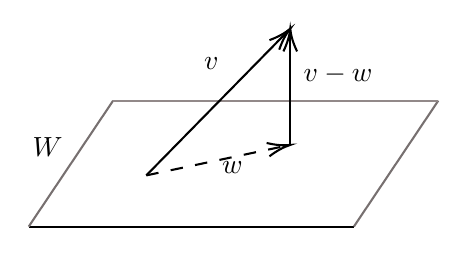
\begin{tikzpicture}[line width=0.75pt,x=0.75pt,y=0.75pt,yscale=-1,xscale=1]
%uncomment if require: \path (0,300); %set diagram left start at 0, and has height of 300

%Straight Lines [id:da5393834497664481]
\draw    (243.67,176.33) -- (400.33,176.33) ;
%Straight Lines [id:da3722628427371233]
\draw [color={rgb, 255:red, 119; green, 112; blue, 112 }  ,draw opacity=1 ]   (441,115.67) -- (400.33,176.33) ;
%Straight Lines [id:da3450034348492136]
\draw [color={rgb, 255:red, 119; green, 112; blue, 112 }  ,draw opacity=1 ]   (284.33,115.67) -- (243.67,176.33) ;
%Straight Lines [id:da008667807992642218]
\draw [color={rgb, 255:red, 146; green, 137; blue, 137 }  ,draw opacity=1 ]   (284.33,115.67) -- (441,115.67) ;
%Straight Lines [id:da7535511013685741]
\draw    (300.33,151.67) -- (368.27,82.43) ;
\draw [shift={(369.67,81)}, rotate = 134.45] [color={rgb, 255:red, 0; green, 0; blue, 0 }  ][line width=0.75]    (10.93,-3.29) .. controls (6.95,-1.4) and (3.31,-0.3) .. (0,0) .. controls (3.31,0.3) and (6.95,1.4) .. (10.93,3.29)   ;
%Straight Lines [id:da6442159524815249]
\draw  [dash pattern={on 4.5pt off 4.5pt}]  (300.33,151.67) -- (367.71,137.41) ;
\draw [shift={(369.67,137)}, rotate = 168.06] [color={rgb, 255:red, 0; green, 0; blue, 0 }  ][line width=0.75]    (10.93,-3.29) .. controls (6.95,-1.4) and (3.31,-0.3) .. (0,0) .. controls (3.31,0.3) and (6.95,1.4) .. (10.93,3.29)   ;
%Straight Lines [id:da8845013680805118]
\draw    (369.67,137) -- (369.67,83) ;
\draw [shift={(369.67,81)}, rotate = 90] [color={rgb, 255:red, 0; green, 0; blue, 0 }  ][line width=0.75]    (10.93,-3.29) .. controls (6.95,-1.4) and (3.31,-0.3) .. (0,0) .. controls (3.31,0.3) and (6.95,1.4) .. (10.93,3.29)   ;

% Text Node
\draw (326.67,93.4) node [anchor=north west][inner sep=0.75pt]    {$v$};
% Text Node
\draw (244,131.73) node [anchor=north west][inner sep=0.75pt]    {$W$};
% Text Node
\draw (335.33,143.4) node [anchor=north west][inner sep=0.75pt]    {$w$};
% Text Node
\draw (374.67,97.07) node [anchor=north west][inner sep=0.75pt]    {$v-w$};
\end{tikzpicture}
\end{center}

\begin{prop}
    For any $v \in V$, there exists a unique orthogonal projection of $v$ onto $W$, denoted $\proj_W(v)$
\end{prop}

\begin{proof}
    Let $e_1,\dots,e_k$ be an orthonormal basis of $W$, and we're looking for a specific $w = \lambda_1e_1+\cdots +\lambda_ke_k$. In particular, we require $(w-v) \perp e_i$ for all $i$, hence
    $$0=\angles{\lambda_1e_1+\cdots +\lambda_ke_k-v,e_i}=\lambda_i-\angles{v,e_i} \iff \lambda_i=\angles{v,e_i}.$$
    This gives us uniquely determined coefficients, namely
    $$\proj _W(v) = \sum_{i=1}^k\angles{v,e_i}e_i$$
\end{proof}

\begin{defn}
    The \textbf{orthogonal compliment} of a subspace $W$ is
    $$W^\perp = \{v \in V \mid \angles{v,w}=0,w \in W\}$$
\end{defn}

\begin{prop}
    $V = W \oplus W^\perp$
\end{prop}

\section{Orthogonal and Unitary Transformations}

\begin{defn}
    Let $F = \R$ (resp. $\C$), and equip $F^n$ with the standard (resp. hermitian) inner product. We say $A \in M_n(F)$ is \textbf{orthogonal} (resp. \textbf{unitary}) if its columns form an orthonormal basis of $F^n$
\end{defn}

\begin{defn}
    The \textbf{adjoint} of a matrix $A$ is defined to be $A^*:=\bar A^t$.
\end{defn}

\begin{thm}
    Let $A \in M_n(F)$. Then, TFAE
    \begin{enumerate}[(i)]
        \item $A$ is orthogonal/unitary
        \item $AA^*=A^*A=I$
        \item $A$ preserves the inner product, i.e. $\angles{Ax,Ay}=\angles{x,y}$.
        \item $A$ is a \textbf{linear isometry}, meaning it preserves distance, i.e. $d(Ax,Ay)=d(x,y)$.
    \end{enumerate}
\end{thm}

\begin{proof}
    Exercise.
\end{proof}

As usual, we can extend the notion of unitary and orthogonal matrices to linear maps.

\begin{defn}
    If $V$ is a standard (resp. hermitian) inner product space, we say $T\in \Hom(V,V)$ is orthogonal (resp. unitary) if $\angles{Tx,Ty}=\angles{x,y}$ for all $x,y \in V$. This is equivalent to $(T)_B$ being orthogonal (resp. unitary) with respect to any orthonormal basis $B$.
\end{defn}

\begin{ex}
    Let $A \in M_n(\R)$ be orthogonal, so $AA^t=I$. It's known that $\det (A) = \det (A^t)$, hence $\det (A)^2=\det (I)=1$, therefore $\det (A) = \pm 1$. We say $A$ is \textbf{orientation preserving} if $\det (A)= 1$, and $A$ is \textbf{orientation reversing} if $\det (A) = -1$.

    Now, consider the case when $A \in M_2(\R)$, letting $A = \matr{Ae_1 & Ae_2}.$ As the columns are assumed to be orthonormal, we know that if the first column is $(x,y)$, then $x^2+y^2=1$. It follows that $x = \cos \theta$ and $y = \sin \theta$ for some $\theta \in \R$. It then follows by the necessary othonormality of the columns that either
    \begin{enumerate}
        \item[(a)] $Ae_2 = \matr{- \sin \theta \\ \cos \theta}$, so $A$ is the orientation preserving rotation by $\theta$
        \item[(b)] $Ae_2=\matr{\sin \theta \\ - \cos \theta}$, so $A$ is the orientation reversing reflection about some line.
    \end{enumerate}
\end{ex}

Recall the definition of an isometry from earlier:

\begin{defn}
    An \textbf{isometry} or \textbf{rigid motion} $m: \R^n \to \R^n$ is a function that preserves distances. That is, $d(m(a),m(b)) = d(a,b)$ for all $a,b \in \R^n$.
\end{defn}

\begin{thm}
    \begin{enumerate}
        \item[(a)] An isometry $m:\R^n \to \R^n$ with $m(0)=0$ is linear. Hence, it is left multiplication by some orthogonal matrix.
        \item[(b)] Furthermore, every isometry of $\R^n$ is the composition of an orthogonal map and a translation $\tau _v$ for some $v \in \R^n$ (so $\tau_v(x)=x+v$)
    \end{enumerate}
\end{thm}
